\chapter{Исследовательская часть}

\section{Технические характеристики}

Технические характеристики устройства, на котором выполнялись замеры по времени представлены далее.

\begin{itemize}
	\item Процессор: Intel(R) Core(TM) i5-10300H CPU @ 2.50 ГГц 2.50 ГГц. \cite{intel}
	\item Оперативная память: 16 ГБ.
	\item Операционная система: Windows 11 Pro 64-разрядная система версией 22H2. \cite{windows}
\end{itemize}

При замерах времени ноутбук был включен в сеть электропитания и был нагружен только системными приложениями.

\clearpage

\section{Демонстрация работы программы}

На рисунке \ref{img:demonstration} показано консольное меню, разработанного приложения для работы с алгоритмами умножения матриц и для измерение работы алгоритмов умножения матриц.

\begin{figure}[h]
	\centering
	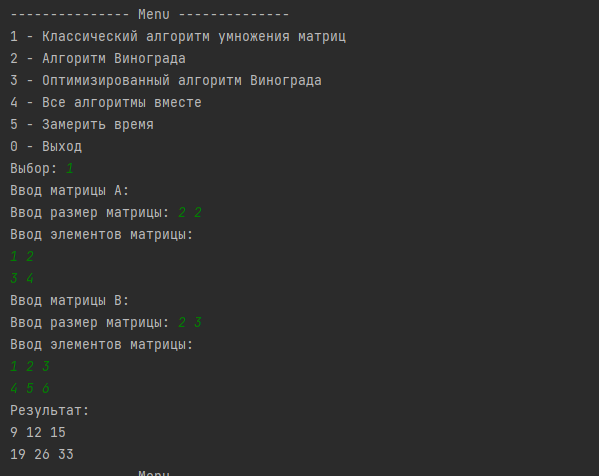
\includegraphics[height=0.5\textheight]{img/example.png}
	\caption{Демонстрация работы программы}
	\label{img:demonstration}
\end{figure}

\clearpage

\section{Временные характеристики}

Результаты эксперимента замеров по времени приведены в \newline
Таблицах \ref{tbl:even_time}, \ref{tbl:odd_time}.

В Таблице \ref{tbl:even_time} приведены результаты замеров по времени алгоритмов умножения матриц при четных размеров квадратных матриц,  размеров \newline от 10 до 100 по 1000 раз на различных входных матрицах.

\begin{table}[ht]
	\small
	\begin{center}
		\begin{threeparttable}
		\caption{Результаты замеров времени (чётные размеры матриц)}
		\label{tbl:even_time}
		\begin{tabular}{|c|c|c|c|}
			\hline
			& \multicolumn{3}{c|}{\bfseries Время, мс} \\ \cline{2-4}
			\bfseries Размер матрицы & \bfseries Классический & \bfseries Винограда & \bfseries (опт.) Винограда
			\csvreader{csv/even_time.csv}{} 
			{\\\hline \csvcoli & \csvcolii & \csvcoliii & \csvcoliv} \\
			\hline
		\end{tabular}	
		\end{threeparttable}
	\end{center}
\end{table}

По таблице \ref{tbl:even_time} был построен график \ref{plt:even_comp_alg}. Исходя из этих данных можно понять, что лучшего всего работает оптимизированный алгоритм Винограда, а классический алгоритм работаем в 1,5 раз хуже, чем алгоритм Винограда.

\clearpage

\begin{figure}[h]
	\centering
	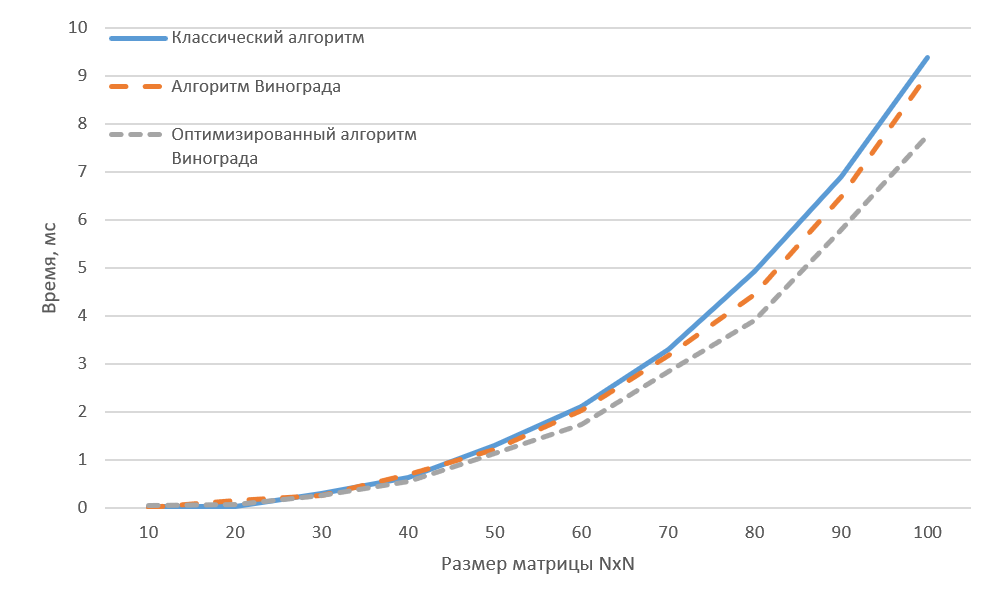
\includegraphics[height=0.3\textheight]{img/comp_alg_even_all.png}
	\caption{Сравнение по времени алгоритмов умножения матриц на чётных размерах матриц}
	\label{plt:even_comp_alg}
\end{figure}

В Таблице \ref{tbl:odd_time} приведены результаты замеров по времени алгоритмов умножения матриц при нечетных размеров квадратных матриц, размеров \newline от 11 до 101 по 1000 раз на различных данных.

\begin{table}[ht]
	\begin{center}
		\begin{threeparttable}
		\small
		\caption{Результаты замеров времени (нечётные размеры матриц)}
		\label{tbl:odd_time}
		\begin{tabular}{|c|c|c|c|}
			\hline
			& \multicolumn{3}{c|}{\bfseries Время, мс} \\ \cline{2-4}
			\bfseries Размер матрицы & \bfseries Классический & \bfseries Винограда & \bfseries (опт.) Винограда
			\csvreader{csv/odd_time.csv}{}
			{\\\hline \csvcoli & \csvcolii & \csvcoliii & \csvcoliv} 
			\\
			\hline
		\end{tabular}
		\end{threeparttable}
	\end{center}
\end{table}

\clearpage

По таблице \ref{tbl:odd_time} был построен графики \ref{plt:odd_comp_alg}. Исходя из этих данных можно понять, что лучшего всего работает оптимизированный алгоритм Винограда, а классический алгоритм работаем в 1,1 раз хуже, чем алгоритм Винограда.

\begin{figure}[h]
	\centering
	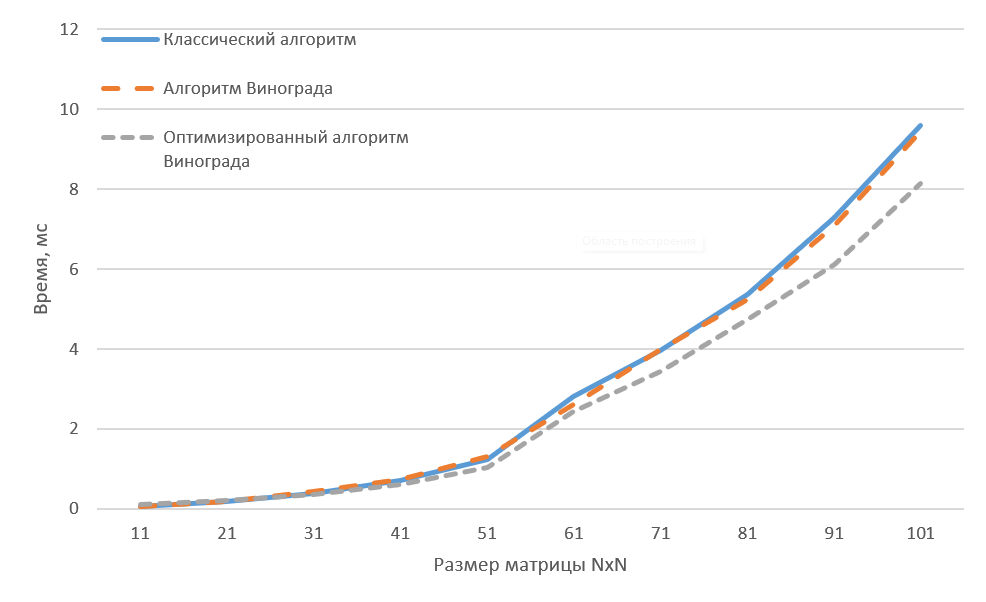
\includegraphics[height=0.3\textheight]{img/comp_alg_odd_all.png}
	\caption{Сравнение по времени алгоритмов умножения матриц на нечётных размерах матриц}
	\label{plt:odd_comp_alg}
\end{figure}


\section{Вывод}
В результате эксперимента было получено, что при больших размерах матриц (свыше 10), алгоритм Винограда быстрее стандартного алгоритма более, чем 1.1 раза, а оптимизированный алгоритм Винограда быстрее стандартного алгоритма в 1.5 раза. В итоге, можно сказать, что при таких данных следует использовать оптимизированный алгоритм Винограда. 

Также при проведении эксперимента было выявлено, что на чётных размерах реализация алгоритма Винограда в 1.1 раза быстрее, чем на нечётных размерах матриц, что обусловлено необходимостью проводить дополнительные вычисления для крайних строк и столбцов. Следовательно, стоит использовать алгоритм Винограда для матриц, которые имеют чётные размеры.
